\chapter{Behavior of gravity waves in water (the ripple tank)}\label{cha:ripple-tank}

%TODO include theoretical limit considerations in curve fitting

\section{Introduction}

The Michelson interferometer, named after University of Chicago professor Albert A. Michelson (Nobel prize in Physics 1907), is an extremely sensitive instrument capable of measuring incredibly tiny displacements.
A modern version of the Michelson interferometer has been developed by The Laser Interferometer Gravitational-Wave Observatory (LIGO) experiment to detect changes in distance of $10^{-19}\:$m (much less than the size of the nucleus of an atom!).
This displacement is sensed between mirrors separated by 4 km (see Figure~\ref{rt:fig:ligo-aerial}). There are two sites for LIGO --- one in Hanford, WA and the other in Livingston, LA.
The LIGO interferometer has recently detected gravitational waves for the first time (September 15, 2015); the first announced gravitational wave detection fits, with remarkable precision, the expected signal from the merging of two black holes, 29 and 36 solar masses, located 410 Mpc away.
The reported signal and the comparison to the fitted model are shown in Figure~\ref{rt:fig:ligo-signals}.

\begin{figure}
	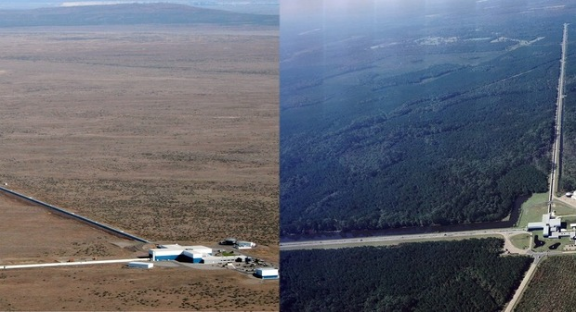
\includegraphics[width=\textwidth]{ripple-tank/ligo-aerial.png}
	\caption{An aerial view of the two LIGO sites.}\label{rt:fig:ligo-aerial}
\end{figure}

\begin{figure}
	\centering
	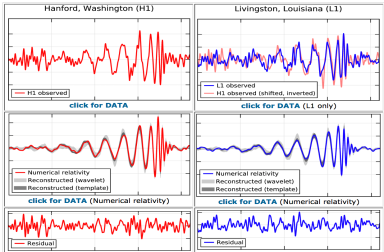
\includegraphics[width=0.7\textwidth]{ripple-tank/ligo-signals.png}
	\caption{The left panels show the LIGO signal at the Hanford site (top) and the best-fit model
		(middle) and the residual of the model minus the data (bottom). The residuals are consistent
		with noise. The right panels show the same for the Livingston site, with the Hanford signal
		plotted in red in the top panel to demonstrate the similarity of the two measurements (as
		expected in the event of a true gravitational wave signal). This first LIGO detection of a
		gravitational wave event marks a significant transformation in our collective ability to
		measure and understand black holes, and since that first detection, more black hole merger
		events have been detected and reported.}\label{rt:fig:ligo-signals}
\end{figure}

The working principle of the Michelson interferometer is the interference of light.
In this lab, you will first explore the concepts of interference with waves produced in water, in a device known as a ripple tank.
In particular, in this first portion of the lab you will experimentally verify a relationship between wave frequency and wavelength, and then demonstrate constructive and destructive wave interference.
You will then extend that understanding of interference to a wave geometry more appropriate to the second portion of the lab.
The final measurement with the ripple tank will allow you to show that plane waves propagating through a slit behave as though the slit were a new source of waves, propagating radially (i.e.\ in a circular pattern).

Next week, you will measure interference phenomena with light, with a modern version of the famous double-slit experiment performed by Thomas Young in 1801.
You will show that the interference properties of waves established in the first section of the lab apply to light as well, thus experimentally demonstrating that light behaves in a wavelike manner.

Having established the wavelike nature of light, you will then finally use a table-top Michelson interferometer to measure changes in distances smaller than a human hair (not quite LIGO sensitivity, but still pretty impressive!).

\section{Learning Goals}

\begin{itemize}
	\item Learn how to conduct an observational experiment, including collecting data and analyzing the data to find and describe a pattern quantitatively.
	
	\item Discover the relationship between frequency and wavelength of waves.
	
	\item Learn how to conduct a testing experiment, including identifying a hypothesis, designing an experiment, making a prediction, and comparing it to an experimental outcome.
	
	\item Gain familiarity with wave interference.
\end{itemize}

\section{An aside: picking a project topic}

By the end of lab today, ensure that you have chosen a topic for your presentation+paper project, and that it has been approved by your TA.

\section{The Scientific Cycle\protect\footnote{adapted from \cite{etkina_college_2014}}}

One way of describing science is the process of incrementally improving a shared model of how our universe works. In different fields of science, different methods and cycles are used, so there is no ``One True Scientific Method.'' One can still create a model for the process of science, and we describe here one such cycle (the hypothetico-deductive cycle), summarized in Figure~\ref{me:fig:isle}.

In this cycle, there are three types of experiments, each one representing a different stage of the scientific effort. One stage, often started when encountering a novel phenomenon, is the \textbf{observational experiment}. This is an experiment that consists of deciding what to observe and how to observe it, collecting data, finding a pattern, and brainstorming possible explanations for what is observed (also called ``hypotheses'').

Once one has some trial explanations, one can test one or more of those with a \textbf{testing experiment}. Here, one designs a new experimental procedure and uses each hypothesis to predict what will happen. Then the prediction is compared to the procedure's outcome. If they are different, then the hypothesis is judged to be not a helpful explanation for that phenomenon. If they are the same, then it is still helpful. Throughout this stage, one may make various assumptions that would need to be validated, as they can effect the prediction or outcome.

Once a hypothesis has been tested enough for people to find it useful, then it can be applied to solve practical problems, or to determine properties of particular situations, in an ``application experiment.''

\begin{figure}
	\centering
	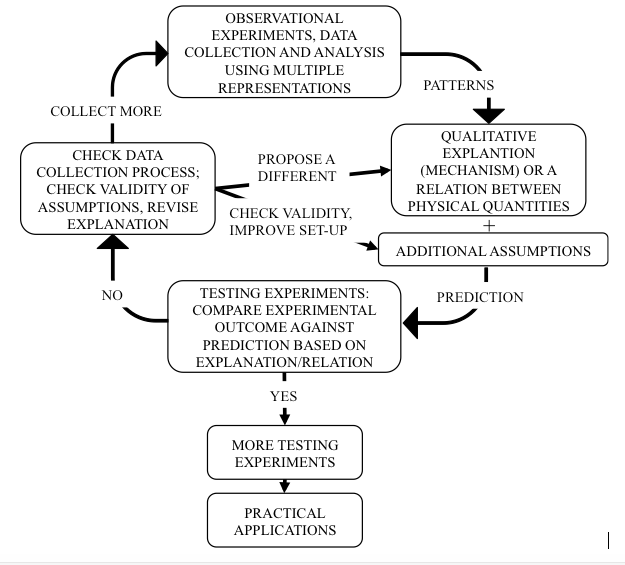
\includegraphics[width=0.7\textwidth]{ripple-tank/islegraphic.png}
	\caption{A model of the process some scientists go through to create knowledge.\cite{etkina_millikan_2015}}\label{me:fig:isle}
\end{figure}

\section{Experiment 1: Observation of frequency and wavelength}

\textbf{Goal:} Observe gravity waves in a ripple tank and determine a mathematical relationship between frequency and wavelength.

\textbf{Available equipment:} ripple tank with strobe light and ripple generator, plane wave attachment, 2 dippers (narrow plastic rods), 1 short wall, 1 medium wall, 2 long walls for ripple tank, flashlights or desk lamps, digital camera (e.g.\ your smartphone), computer with ImageJ installed (can be your device), object of known size to be submerged

\begin{framed}
	\textbf{Caution: Flickering Lights!} You will be using a stroboscopic light in this lab. Such light is known to trigger reactions in some individuals (e.g. photosensitive epilepsy).
	If you are worried that you may be sensitive to strobe light, speak to the TA and skip attending this part of the lab.
	In any case, avoid staring directly at the light.
\end{framed}

\begin{framed}
	\textbf{Self-assessment:} To help you improve your scientific abilities, we provide you with self-assessment rubrics.
	A rubric is a scoring system.
	Self-assessment is determining how well you performed a particular task.
	So, these self-assessment rubrics are designed to help you evaluate your performance while you are designing and performing your experiment.
	
	The complete set of rubrics is available in Appendix~\ref{cha:rubrics}.
	In each lab, your report will be assessed using Rubric F, found in Table~\ref{rubric:f}, as well as 5 additional rubric rows listed in that lab.
	Each week, read through these and use them to evaluate your work as you design and perform the experiment.
	Your instructor will use the same rubrics to determine part of your grade for the lab.
\end{framed}	

\textbf{Rubrics to focus on during this experiment:} B7, B8, F1, F2. See Appendix~\ref{cha:rubrics} for details.

\subsection{The ripple tank and generator}

In this section you will explore interference phenomena using a ripple tank. The tank --- 42.5 cm x 42.5 cm and 2.5
cm deep --- is filled with water, and is equipped with a ripple generator. The generator uses voice coil actuators to
produce the precise and quiet up-and-down motion of the rippler arms. Waves are generated in the tank by the moving
dippers that touch the surface of the water. The generator also controls a light source that produces a bright, clear
image of the wave patterns in the ripple tank. The light can be used as a steady source or as a strobe to ‘freeze’ the
motion of the wave patterns (in this case the flashing light and the generator are driven with the same frequency). The
ripple generator frequency ranges from 1.0 to 50 Hz adjustable in 0.1 Hz increments. You will work with frequencies in
the range 16--32 Hz. A mirror placed below the tank and working in conjunction with a projection screen provide a
magnified image of the wave patterns in the water; you will record patterns seen on this screen by photographing them
with a digital camera. The ripple generator terminates in a bar with numerous clips in which you can place various
``dippers''.

\subsection{Suggestions for your experiment}

\begin{enumerate}
	\item You may want to decide on roles for each group member. Example roles include Facilitator (ensures time and group focus are efficiently used), Scribe (ensures work is recorded), Technician (oversees apparatus assembly, usage), Skeptic (ensures group is questioning itself). Note that each role is responsible for ensuring that the thing happens, rather than necessarily doing it themselves. \textbf{Decide if you are using these roles, and if so, assign them and note them in the lab report.}
	
	\item Ensure that every group member knows what the terms frequency and wavelength mean, in relation to waves. Use whatever means at your disposal to do this.
	
	\item This is an ``observational experiment.'' Review Rubric B (Table~\ref{rubric:b}) and discuss any unclear expectations with your group and the instructor. Note that your lab report will be graded, in part, on demonstration of Abilities B7 and B8.
	
	\item Ensure that one of the ripple tank's ripple generator is set up with 1 dipper fixed in the center clip of the bar that extends from the box, and that the height of the generator is such that the dipper just touches the top of the water. You can make coarse adjustments by moving the generator along the support rod, and fine adjustments with the two red knobs on it.
	
	\item Brainstorm different methods you could use to determine the relationship between wavelength and frequency. Feel free to play with the ripple tank as you do so, seeing what the frequency and amplitude knobs do. Notice that for different frequencies, different amplitudes produce the clearest image. Here are some things to consider:
	\begin{itemize}
		\item Which variable will you control (and thus will be the independent variable) and which will you measure?
		
		\item What is the range of the independent variable that you will use? How many different settings will you choose?
		
		\item You will need to use several settings of the independent variable, and then plot the data in a graph, decide on what pattern you see, and give some justification for that pattern. You can use words like ``proportional'', ``linear'', ``parabolic'', ``exponential'', ``logarithmic'', and so on, if they fit. Ensure you use the mathematical definition of these.
		
		\item How will you measure the wavelength?
		\begin{itemize}
			\item Is it a more precise measurement if you measure several of them at once and divide to get a single wavelength?
			
			\item The reflected image might magnify the ripple tank, so it can be helpful to place an object of known size in the tank, like a coin, so you can determine the correct scaling.
		\end{itemize}
		
		One way to take careful measurements of the wavelength is to take a picture of the projected tank, then use a program like ImageJ to measure the lengths you need. If you do so, one way to keep track of what settings go with what image is to mark a card with the settings and place it in view of the camera. See the section below on measuring lengths with ImageJ.
	\end{itemize}

	\item Decide on your measurement and analysis method and discuss it with an instructor before you begin. They will help increase the chances that your method will lead to successful results, or at least that the unhelpful path that you choose will take a short enough amount of time for you to change it when you discover it does not work. We want you to have productive failure that you have time to learn from.
	
	\item Perform your experiment. Your lab report for this experiment should include:
	\begin{itemize}
		\item A labeled sketch or photo of the setup, and a description of the experimental procedure (see Rubric F1).
		
		\item A plot of wavelength vs. frequency (with the independent variable on the horizontal axis)
		
		\item A description of the pattern found. This can be done with a line (straight or curved) showing the pattern you see (either drawn manually or using the curve fitting function of the plotting program, e.g.\ LibreOffice Calc or Microsoft Excel) and with words describing what you found. (B7)
		
		\item An equation to represent the pattern. This can be taken from a curve fit or found by hand. Make sure there is some discussion of how well the equation agrees with the data, but you don't need to be very precise about it. (B8)
		
		\item A discussion of the findings of the experiment and why it's helpful (for you and/or for science) (F2)
	\end{itemize}

\end{enumerate}

\subsection{Measuring lengths using ImageJ}

ImageJ (\url{http://imagej.nih.gov/ij/download.html}), which is installed on the lab computers, is useful for measuring lengths in images. To do so, load your image, then follow these steps to calibrate the ruler --- that is, to tell ImageJ how long something is in the image, so it knows how many pixels correspond to what length).

\begin{enumerate}
	\item Start with an image that has an object in it that you know one of the lengths of (e.g.\ the length of side, or a diameter).
	
	\item Open that image in ImageJ.
	
	\item Select the icon with the straight line on it, and click and drag along the known length.
	
	\item From the drop-down menu, select ``Analyze'' $>$ ``Set Scale...''.
	
	\item Set ``Known distance'' to the value of the known length.
	
	\item Set ``Unit of length'' to the unit you are using, for example ``mm'' for millimeters.
	
	\item Record the pixel scale given at the bottom of the box for future use.
	
	\item Now when you use the straight line tool, it will give the length in physical units in ImageJ's toolbar.
\end{enumerate}

\section{Experiment 2: Testing the conditions for constructive interference}

\textbf{Goal:} Test the hypothesis that constructive interference between two waves occurs at positions where the distance from each source differs by a half-integer number of wavelengths, or
\begin{equation}
 \Delta d = (m+\frac{1}{2})\lambda \,,
\end{equation}
where $\Delta d$ is the ``path length difference'', $\lambda$ is the wavelength, and $m$ is any integer.

\textbf{Available equation:} Same as in the previous experiment.

\textbf{Setup:} Instead of 1 dipper, use two dippers mounted with 3 empty clips between them on the bar. Ask the TA for assistance in setting this up. Adjust so that the dippers are just resting in the surface of the water. Adjust the frequency and amplitude to get clear, sharp waves.

\textbf{Rubric rows to be assessed in this experiment:} C1, C4, C7, F1, F2. See Appendix~\ref{cha:rubrics} for details.

\subsection{Testing this hypothesis}

In general, one tests a hypothesis by using it to make a prediction about what will happen in a certain experimental procedure. With this hypothesis, it asserts a relationship between path length difference, wavelength, and constructive interference. But there are only certain points on the ripple tank image where it is easy to see constructive interference --- the bright spots at the intersection of waves originating from both sources. For an example, see Figure~\ref{rt:fig:interference-2d}.

\begin{figure}
	\centering
	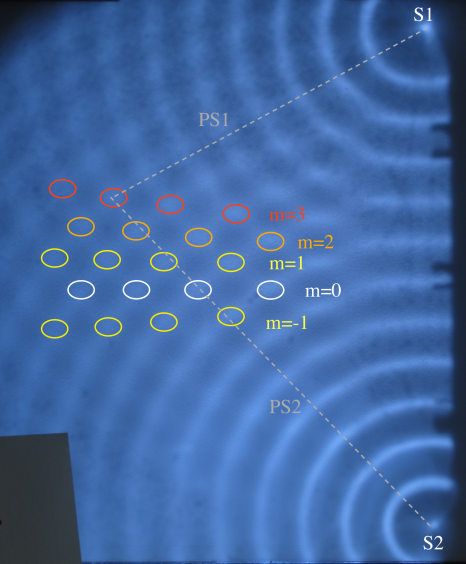
\includegraphics[width=0.7\textwidth]{ripple-tank/interference-2d.png}
	\caption{Example interference pattern for 2 dippers. The bright spots are circled. For a particular bright spot of constructive interference, the two path lengths PS1 and PS2 are drawn.}\label{rt:fig:interference-2d}
\end{figure}

In this case, it is easier to start by finding those locations, measuring the $\Delta d$, finding the wavelength for the given frequency using the relationship you found in Experiment 1, and solving for $m$. The hypothesis predicts that $m$ should always be an integer. As a result, your experiment becomes this: find out how close the experimentally determined $m$'s are to integers.

Brainstorm your experimental procedure, decide on it, discuss with your TA, then perform the experiment.

Your lab report for this experiment should include:
\begin{itemize}
	\item A clear description of the hypothesis (see Rubric C1).
	
	\item A labeled sketch or photo of the setup, and a description of the experimental procedure (F1).
	
	\item A clear statement of the prediction that the hypothesis makes for this particular procedure (C4).

	\item A table of path lengths, path length differences, and measured $m$ values.
	
	\item An analysis of how close the measured $m$ values are to the prediction. Use some quantitative measure of this, but don't worry about being precise about uncertainties (C7).
	
	\item A judgment about the hypothesis. Is it supported, disproved, or undetermined? (C8, though not assessed this time)
	
	\item A discussion of the findings of the experiment and why it's helpful (for you and/or for science) (F2).
\end{itemize}

%In the case of a hypothesis like this one, that includes a proposed equation, there is a useful template for coming up with a prediction:
%\begin{enumerate}
%	\item Note that this hypothesis is asserting that when the equation is true, there is constructive interference (a bright spot). So the goal is to test how true this is.
%	
%	\item Choose which variables you are holding constant, which one is the independent, and which is the dependent variable. In this case, you may not know what $m$ is ahead of time. You could choose it arbitrarily, for example $m=0$ first, and go from there.
%	
%	\item Once you decide on your procedure (which things to measure, how to vary the independent variable), you can use the equation to solve for the dependent variable, which becomes the prediction (Rubric C4).
%	
%	\item The set of dependent variables (for each chosen independent variable) becomes the prediction of the hypothesis that you will use to compare to experimental outcome (C7).
%\end{enumerate}
%
%\subsection{Suggestions for your experiment}
%
%\begin{itemize}
%	\item Note that constructive interference happens where there are bright spots in the projected image at the intersection of waves coming from both sources.
%	
%	\item There is an entire line of points that have the same path length difference from each source, so for each choice of $m$, there can be many 
%\end{itemize}

\section{Experiment 3: Observing plane waves encountering narrow gaps}

This experiment does not clearly follow the model of the scientific cycle, but is closest to an observational experiment. In next week's lab, you will investigate the properties of light traveling through small slits. Ripples in water are more obviously waves, so it is helpful to observe what happens here first.

Instead of dippers, remove them and position the bar so that it is resting in the water. This will produce straight line waves, or, in two dimensions, ``plane waves''. This is the same kind of waves we will use next week with light.

Adjust the amplitude and frequency, with the frequency in the range 20--25 Hz, until you see
clear well-defined vertical parallel lines. Now, insert the two large ``walls'' in the tank, parallel to the rippler bar and
perhaps 5cm away; allow a small (few mm) opening between the two wall sections, placed so that opening is vertically
centered in the projected image. Adjust the amplitude upward until you see a clear wave pattern radiating from that
opening. Take a picture. Repeat this with two apertures instead of one; do this by adding a smaller wall between the
two larger sections, with all sections parallel to the rippler bar, and a small gap between each larger wall and the central
smaller portion. Again, take a picture, adjusting amplitude as necessary to get well-defined waves.

The analysis of this will be done as individual homework.

\section{Individual Homework}

These questions are to be answered individually and your answers should be submitted under the Lab 1 Homework assignment on Canvas.

Both questions concern the last two situations recorded in the lab: the case of 2 walls (1 gap or ``aperture'') and the case with 3 walls (2 apertures).

\begin{enumerate}
	\item What wave pattern do you see in the case of a single aperture? What do you see In the case of a double aperture?
	How do these patterns compare to the data you took using dippers on the rippler bar?
	
	\item Is the wavelength of the pattern you observe consistent with the relationship between frequency and wavelength you
	measured with the dippers? Include any measurements and calculations you make in answering this question in your homework response, and be quantitative.
\end{enumerate}